\documentclass[tikz,border=2pt]{standalone}
\usepackage{amsmath,amssymb}
\usepackage{tikz}
\usetikzlibrary{arrows.meta}

\begin{document}
% The sum of two planes through the origin in R^3 is all of R^3; their intersection is a line,
% so the decomposition w = v1 + v2 is not unique (the sum is not direct).
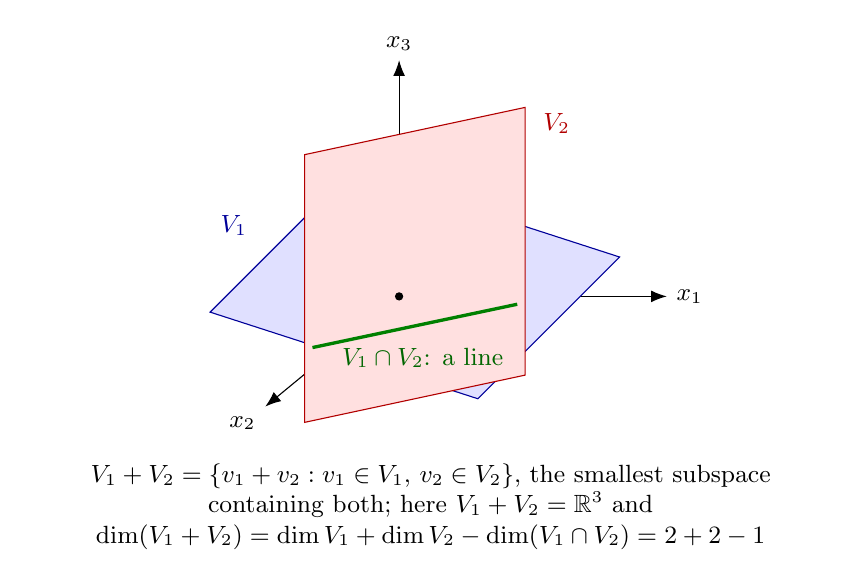
\begin{tikzpicture}[every node/.style={font=\small}, >={Latex[length=2mm]}]
	\draw[->] (0,0) -- (3.4,0) node[right] {$x_1$};
	\draw[->] (0,0) -- (0,3.0) node[above] {$x_3$};
	\draw[->] (0,0) -- (-1.7,-1.4) node[below left] {$x_2$};
	\fill[blue!12] (-2.4,-0.2) -- (1.0,-1.3) -- (2.8,0.5) -- (-0.6,1.6) -- cycle;
	\draw[blue!60!black] (-2.4,-0.2) -- (1.0,-1.3) -- (2.8,0.5) -- (-0.6,1.6) -- cycle;
	\fill[red!12] (-1.2,-1.6) -- (1.6,-1.0) -- (1.6,2.4) -- (-1.2,1.8) -- cycle;
	\draw[red!70!black] (-1.2,-1.6) -- (1.6,-1.0) -- (1.6,2.4) -- (-1.2,1.8) -- cycle;
	\draw[green!50!black, very thick] (-1.1,-0.65) -- (1.5,-0.1);
	\node[blue!60!black, font=\small] at (-2.1,0.9) {$V_1$};
	\node[red!70!black, font=\small] at (2.0,2.2) {$V_2$};
	\node[green!40!black, font=\small] at (0.3,-0.78) {$V_1\cap V_2$: a line};
	\fill (0,0) circle (1.5pt);
	\node[anchor=north, align=flush center, text width=10cm] at (0.4,-2.0) {$V_1+V_2=\{v_1+v_2: v_1\in V_1,\,v_2\in V_2\}$, the smallest subspace containing both; here $V_1+V_2=\mathbb{R}^3$ and $\dim(V_1+V_2)=\dim V_1+\dim V_2-\dim(V_1\cap V_2)=2+2-1$};
\end{tikzpicture}
\end{document}
